\documentclass[11pt, a4paper]{article}


% Modules essentiels
\usepackage[french]{babel}
\usepackage[T1]{fontenc}
\usepackage[hmargin=2.5cm, vmargin=2.5cm]{geometry}
\usepackage[utf8]{inputenc}
\usepackage[skip=1em]{parskip}


% Modules supplémentaires
\usepackage[algoruled, lined, linesnumbered, longend, french, frenchkw]{algorithm2e}
\DontPrintSemicolon
\SetNlSty{tiny texttt}{}{}

\usepackage{amsfonts}
\usepackage{amsmath}
\usepackage{amssymb}

\usepackage{caption}

\usepackage{color}
\definecolor{mybordeaux}{rgb}{0.43, 0.03, 0.01}
\definecolor{mygray}{rgb}{0.95, 0.95, 0.95}
\definecolor{mygreen}{rgb}{0, 0.6, 0}
\definecolor{myred}{rgb}{0.6, 0, 0}
\definecolor{mypurple}{rgb}{0.73, 0.33, 0.83}

\usepackage{enumitem}
\setlist[itemize]{noitemsep, left=11pt}

\usepackage{graphicx}
\graphicspath{{../images}}

\usepackage{hyperref}
\addto\extrasfrench%
{%
	\def\algorithmautorefname{\textsc{Alg.}}
	\def\equationautorefname{\textsc{Éq.}}
	\def\figureautorefname{\textsc{Fig.}}
	\def\lstlistingautorefname{\textsc{List.}}
	\def\sectionautorefname{\textsc{Sec.}}
	\def\subsectionautorefname{\textsc{Sec.}}
	\def\subsubsectionautorefname{\textsc{Sec.}}
	\def\tableautorefname{\textsc{Tab.}}%
}

\usepackage{listings}
\lstset%
{%
	basicstyle=\ttfamily,
	backgroundcolor=\color{mygray},
	breaklines=true,
	captionpos=b,
	commentstyle=\color{mygreen},
	emph={},
	emphstyle=\color{mybordeaux},
	extendedchars=true,
	firstnumber=1,
	frame=single,
	keywordstyle=\color{myred},
	language=Python,
	literate= {À}{{\`A}}1 {à}{{\`a}}1 {é}{{\'e}}1 {è}{{\`e}}1,
	numbers=left,
	numberstyle=\tiny\color{black},
	showstringspaces=true,
	stepnumber=5,
	stringstyle=\color{mypurple},
	tabsize=4%
}

\usepackage[version=4]{mhchem}

\usepackage[space-before-unit, per-mode=power, inter-unit-product=.]{siunitx}

\usepackage{subcaption}

\usepackage{tabularx}


% Caractéristiques du document
\title{Démarche adoptée pour la préparation d'une configuration plus complexe}
\author{Heiarii Lou Chao}
%\date{}


\begin{document}
\maketitle
\tableofcontents

\clearpage
\section*{Introduction}

Nous souhaitons effectuer des simulations sur des structures plus complexes que l'exemple précédent (LAMMPS Lennard-Jones), pour cela nous préparons la simulation de molécules d'eau réparties dans une boîte.

\section{Préparation de la configuration}

Pour préparer la configuration, nous suivons une démarche similaire à la précédente -- celle adoptée pour la structure graphite + eau -- et nous utilisons PACKMOL.

Les dimensions de la boîte de simulation sont : \fbox{$X = Y = Z = \qty{20.0}{\angstrom}$}.

En prenant $\rho_{\ce{H2O}} = \qty{1000}{\kg \per \cubic \meter}$, $\mathcal{N}_A = \qty{6.022e+23}{\per \mol}$ et $M_{\ce{H2O}} = \qty{1.801e-02}{\kg \per \mol}$, nous trouvons le nombre de molécules d'eau à répartir dans la boîte de simulation : \fbox{$N \approx \num{267}$}.

Comme précédemment, nous prendrons une tolérance de \fbox{$\mathtt{tol} = \qty{1.5}{\angstrom}$}.

Pour anticiper l'application des conditions aux limites périodiques, nous réduisons la région où répartir les molécules à : \fbox{$X^m = Y^m = Z^m = \qty{0.75}{\angstrom}$ et $X^M = Y^M = Z^M = \qty{19.25}{\angstrom}$}.

Le script PACKMOL est présenté au \autoref{lst:packmol}.

\begin{lstlisting}[caption={Répartition des molécules d'eau}, label={lst:packmol}]
tolerance 1.5
output init.xyz
filetype xyz
structure water.xyz
	number 7
	inside box 0.75 0.75 0.75 19.25 19.25 19.25
end structure
\end{lstlisting}

Celui-ci donne la configuration optimisée de la \autoref{fig:initiale}.

\begin{figure}[hbpt]
	\centering
	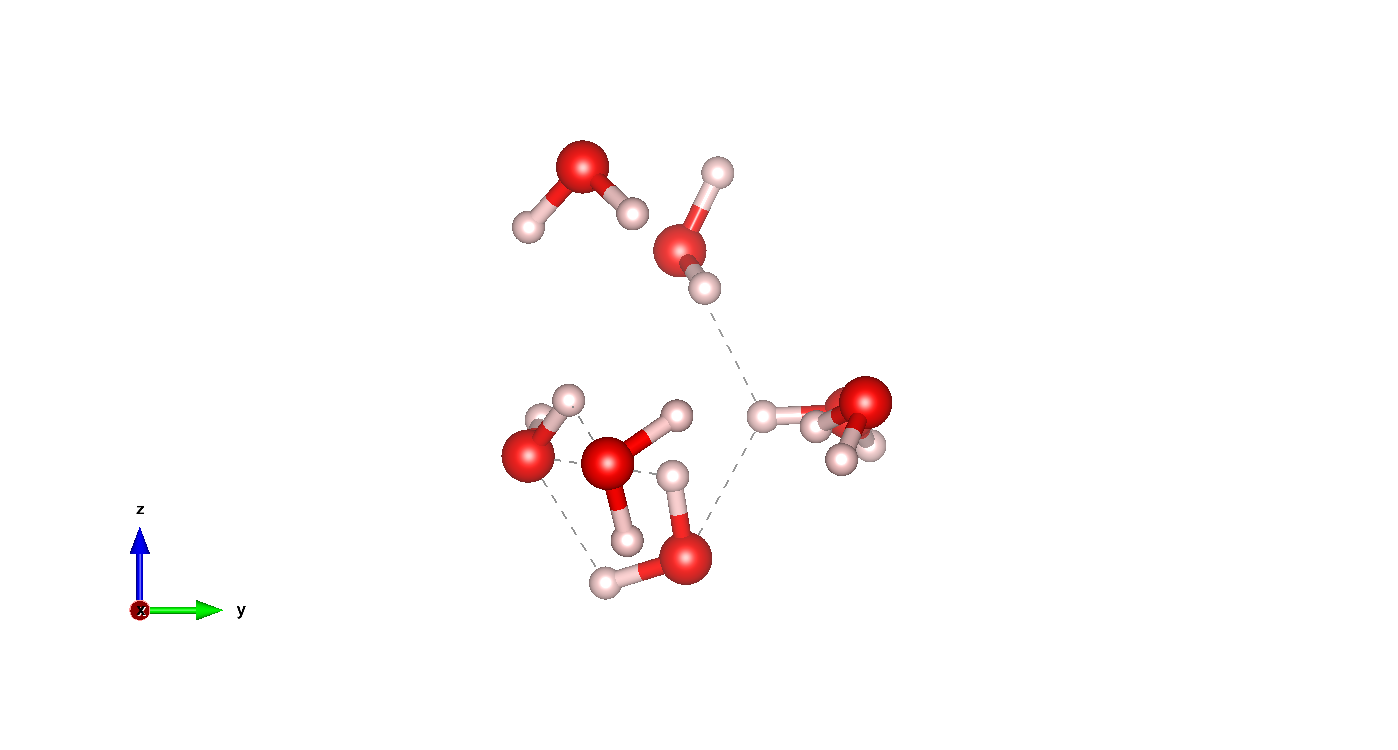
\includegraphics[width=\linewidth]{init.png}
	\caption{Configuration initiale des molécules d'eau}
	\label{fig:initiale}
\end{figure}

\clearpage
\section{Détermination des listes de molécules et de liaisons}

Pour effectuer des simulations de systèmes tels que le précédent, il est nécessaire de fournir un fichier de données à LAMMPS. Celui-ci doit se présenter sous un format spécifique et contenir les informations du système (\href{https://docs.lammps.org/read_data.html#format-of-a-data-file}{manuel utilisateur de LAMMPS}).

Il est donc nécessaire de pré-traiter les données fournies par le fichier XYZ produit par PACKMOL pour les formater et les soumettre à LAMMPS.

	\subsection{Format du fichier de données LAMMPS}

		\subsubsection{En-tête du fichier}

L'en-tête du fichier de notre simulation doit comprendre les champs suivants :
\begin{itemize}
	\item \lstinline!atoms!, le nombre d'atomes
	\item \lstinline!bonds!, le nombre de liaisons
	\item \lstinline!angles!, le nombre d'angles
	\item \lstinline!atom types!, le nombre de types d'atomes
	\item \lstinline!bond types!, le nombre de types de liaisons
	\item \lstinline!angle types!, le nombre de types d'angles
	\item \lstinline!xlo xhi!, les limites de la boîte selon l'axe $[Ox)$
	\item \lstinline!ylo yhi!, les limites de la boîte selon l'axe $[Oy)$
	\item \lstinline!zlo zhi!, les limites de la boîte selon l'axe $[Oz)$
\end{itemize}
où chaque ligne doit se présenter sous la forme
\begin{lstlisting}
value(s)	keyword(s)
\end{lstlisting}

		\subsubsection{Corps du fichier}

Le corps du fichier de notre simulation doit comprendre les sections suivantes :
\begin{itemize}
	\item \lstinline!Masses!, avec le format
\begin{lstlisting}
atom-type	mass
\end{lstlisting}
	\item \lstinline!Atoms!, avec le format \lstinline!full!
\begin{lstlisting}
atom-ID 	molecule-ID 	atom-type	q	x	y	z
\end{lstlisting}
	\item \lstinline!Angles!, avec le format
\begin{lstlisting}
angle-ID	angle-type	atom1	atom2	atom3
\end{lstlisting}
	\item \lstinline!Bonds!, avec le format
\begin{lstlisting}
bond-ID 	bond-type	atom1	atom2
\end{lstlisting}
\end{itemize}

	\subsection{Traitement des données}

Pour le traitement des données, il est important de se rendre compte que les données suivantes doivent être renseignées par l'utilisateur :
\begin{itemize}
	\item le nombre de types d'atomes
	\item le nombre de types de liaisons
	\item le nombre de types d'angles
	\item les limites de l'espace
	\item les correspondances types d'atomes-masses
	\item les correspondances types d'atomes-charges
\end{itemize}

Et les données restantes doivent être déterminées par un script :
\begin{itemize}
	\item le nombre d'atomes
	\item le nombre de liaisons
	\item le nombre d'angles
	\item les positions des atomes
	\item les atomes mis en jeu pour les liaisons
	\item les atomes mis en jeu pour les angles
\end{itemize}

Enfin, le diagramme de la \autoref{fig:donnees_flux} nous permet de dire qu'il faudra déterminer les données du corps du fichier avant de déterminer les données de l'en-tête.

\begin{figure}[hpbt]
	\centering
	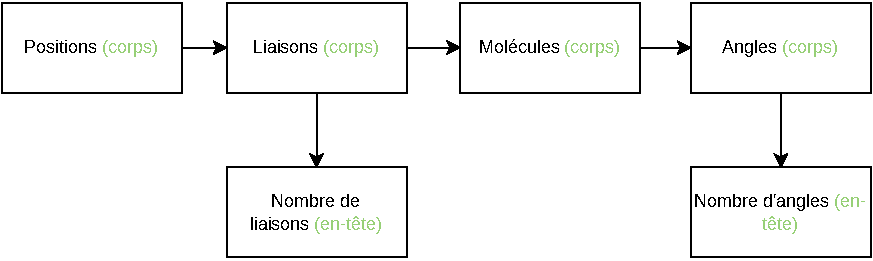
\includegraphics[scale=1]{donnees-flux.pdf}
	\caption{Détermination des éléments du fichier de données}
	\label{fig:donnees_flux}
\end{figure}

		\subsubsection{Détermination des liaisons}

Pour déterminer les liaisons entre les atomes du système nous nous basons sur les distances inter-atomiques. Ceci nous permet de concevoir le diagramme de la \autoref{fig:donnees_liaisons} et l'\autoref{alg:liaisons}.

\begin{figure}[hpbt]
	\centering
	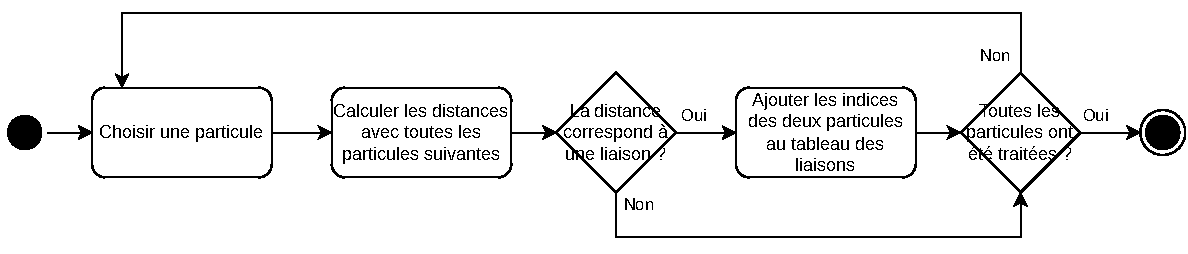
\includegraphics[width=\linewidth]{donnees-liaisons.pdf}
	\caption{Détermination des liaisons}
	\label{fig:donnees_liaisons}
\end{figure}

\begin{algorithm}[htpb]
	\Donnees{$\mathtt{N_{part}}$ le nombre de particules, $\mathtt{r}$ les positions des particules, $\mathtt{N_{tliaisons}}$ le nombre de types de liaisons, $\mathtt{t}$ les seuils des liaisons}
	\Sortie{$\mathtt{L}$ le tableau des indices des paires de particules liées}
	\Deb%
	{
		\Pour{\upshape \bfseries $\mathtt{i}$ de \num{0} à $\mathtt{N_{part}}$}%
		{
			\Pour{\upshape \bfseries $\mathtt{j}$ de $\mathtt{i + 1}$ à $\mathtt{N_{part}}$}%
			{
				$\mathtt{r_{ij} \gets |r_i - r_j|}$\;
				\Pour{\upshape \bfseries $\mathtt{k}$ de \num{0} à $\mathtt{N_{tliaisons}}$}%
				{
					\Si{$\mathtt{t_k} \leq \mathtt{r_{ij}} \leq \mathtt{t_{k + 1}}$}%
					{
						\texttt{ajouter}$\mathtt{(L_k, [i, j])}$\;
					}
				}
			}
		}
		\Retour{$\mathtt{L}$}
	}
	\caption{Détermination des liaisons}
	\label{alg:liaisons}
\end{algorithm}

		\subsubsection{Détermination des molécules}

Pour déterminer les molécules, nous nous basons sur les liaisons en partant du principe qu'une molécule est un ensemble d'atomes liés entre eux au moins deux à deux.\\
Par exemple avec un tableau de liaisons $\mathtt{L = [[[1, 2], [2, 3]]]}$, on veut avoir le résultat $\mathtt{M = [[1, 2, 3]]}$ de sorte à ce que l'entrée $\mathtt{M_0}$ corresponde à la première molécule, mettant en jeu les atomes numérotés \num{1}, \num{2} et \num{3}.

Nous pouvons alors concevoir le diagramme de la \autoref{fig:donnees_molecules} et l'\autoref{alg:molecules}.

\begin{figure}[hpbt]
	\centering
	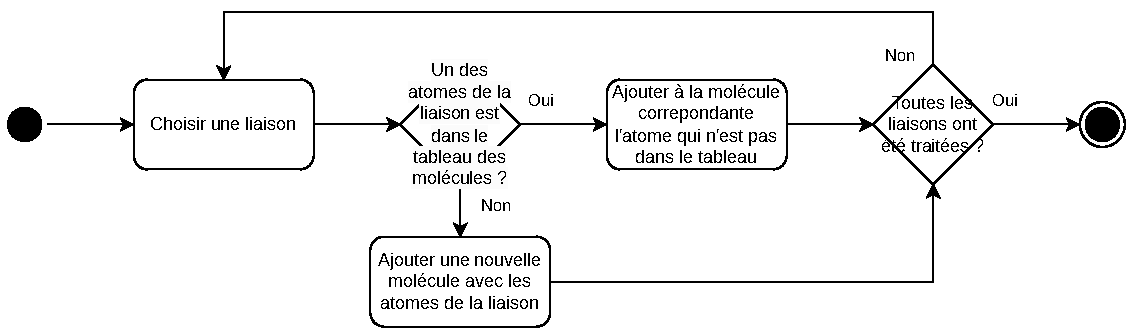
\includegraphics[width=\linewidth]{donnees-molecules.pdf}
	\caption{Détermination des molécules}
	\label{fig:donnees_molecules}
\end{figure}

\begin{algorithm}[hpbt]
	\Donnees{$\mathtt{L}$ le tableau des indices des paires de particules liées}
	\Sortie{$\mathtt{M}$ le tableau des indices des atomes appartenant aux mêmes molécules}
	\Deb%
	{
		$\mathtt{L' \gets concatener(L, axe=0)}$\;
		\Pour{\bfseries \upshape $\mathtt{i}$ de \num{0} à $\mathtt{nombre(L')}$}%
		{
			$\mathtt{ajoute \gets faux}$\;
			\PourCh{\bfseries \upshape $\mathtt{atome}$ de $\mathtt{L'_i}$}%
			{
				\PourCh{\bfseries \upshape $\mathtt{molecule}$ de $\mathtt{M}$}%
				{
					\Si{$\mathtt{atome \in molecule}$}%
					{
						$\mathtt{retirer(L'_i, atome)}$\;
						$\mathtt{ajouter(molecule, L'_i)}$\;
						$\mathtt{ajoute \gets vrai}$\;
						$\mathtt{stopper}$\;
					}
				}
				\Si{$\mathtt{ajoute}$}%
				{
					$\mathtt{stopper}$\;
				}
			}
			\Si{$\mathtt{non~ajoute}$}%
			{
				$\mathtt{ajouter(M, L'_i)}$\;
			}
		}
		\Retour{$\mathtt{M}$}
	}
	\caption{Détermination des molécules}
	\label{alg:molecules}
\end{algorithm}

		\subsubsection{Détermination des angles}

Pour déterminer les angles nous nous basons sur les molécules. Nous pouvons concevoir le diagramme de la \autoref{fig:donnees_angles}, cependant une méthode alternative adaptée pour un système à un type d'angle fonctionne et a été implémentée directement.

\begin{figure}[hbpt]
	\centering
	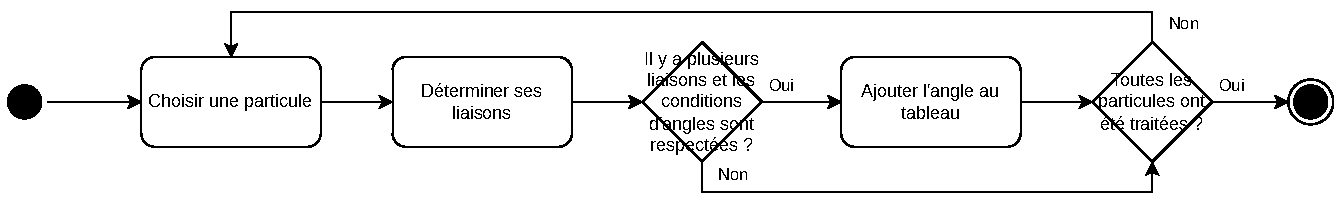
\includegraphics[width=\linewidth]{donnees-angles.pdf}
	\caption{Détermination des angles}
	\label{fig:donnees_angles}
\end{figure}

		\subsubsection{Implémentation}

Ces algorithmes ont pu être implémentés pour construire un script permettant, à partir d'un fichier d'entrée et du fichier de configuration au format XYZ, d'écrire un fichier de données LAMMPS automatiquement.

Le fichier d'entrée doit contenir les informations sur le système à simuler. Un exemple est présenté par le \autoref{lst:conversion_input}.

\begin{lstlisting}[caption={Fichier d'entrée pour la conversion}, label={lst:conversion_input}]
# input.txt
configuration_file: init.xyz
output_file: data.lammps
atom_types: O H
	masses: 15.9994 1.008
	charges: -0.8476 0.4238
bond_types: 1
	thresholds: 0.90 1.00
angle_types: 1
space_boundaries: 0.0 0.0 0.0 6.0 6.0 6.0
\end{lstlisting}

Et le résultat est présenté par un fichier tel que présenté par le \autoref{lst:conversion_sortie}.

\begin{lstlisting}[caption={Fichier de sortie de la conversion}, label={lst:conversion_sortie}]
# data.lammps
LAMMPS Description

  21 atoms
  14 bonds
  ...

Masses

1 15.9994 # O
2 1.008 # H
...

Atoms

1 1 2 0.4238 4.978146 3.160309 2.519717
2 1 1 -0.8476 5.220404 2.390845 1.990387
...

Bonds

1 1 1 2 
2 1 2 3 
...
\end{lstlisting}

\end{document}